\documentclass[12pt]{article}
\usepackage{fullpage}
\usepackage{nopageno}
\usepackage{ifthen}
\usepackage{amsmath}
\usepackage{amssymb}
\usepackage{graphicx} 
\usepackage{version}
\usepackage{amsthm}
\usepackage{multicol}
%\usepackage{add-copyright}

\excludeversion{solution}

\DeclareMathOperator{\ft}{ft}

\newcommand{\R}{\mathbb{R}}

\title{Take-Home Quiz 6}
\author{Math 131 Section 22}
\date{Due Monday, November 21, 2005}

\newcounter{problem}
\setcounter{problem}{1}

\newenvironment{problem}[1][]
{\begin{flushleft}\hangindent=1em\hangafter=1\noindent\textbf{Problem \arabic{problem}.}
\ifthenelse{\equal{#1}{}}{}{
\textbf{(#1 \ifthenelse{\equal{#1}{1}}{point}{points}).}}
}
{\addtocounter{problem}{1}\end{flushleft}}

\begin{document}
\maketitle

These problems illustrate how we can take the material we've learned
to do even fancier things---higher order implicit differentiation and
a totally awesome related rates problem.

\begin{problem}[6]
Consider the equation $x^2 + y^2 = 1$.  Using implicit differentiation
gives a formula for the slope of the tangent line to $(x,y)$ on
the circle with radius one, namely:
$$
2x + 2y \frac{dy}{dx} = 0,
$$
so the tangent line to the point $(x,y)$ has slope $-x/y$.

Use implicit differentiation on this equation to get a formula for
$d^2y/dx^2$.  Do some algebraic manipulation so your formula
for $y''$ only depends on $y$.
\end{problem}

\begin{solution}
\subsection*{Solution}

Differentiating $2x + 2y \frac{dy}{dx} = 0$ with respect to $x$ gives
$$
2 + 2y \frac{d^2 y}{dx^2} + 2 \left( \frac{dy}{dx} \right)^2 = 0.
$$
Solving for the second derivative gives
$$
\frac{d^2 y}{dx^2} = - \frac{1 + \left( \frac{dy}{dx} \right)^2}{y}.
$$
Substituting in the fact that $dy/dx = -x/y$ we get
$$
\frac{d^2 y}{dx^2} = - \frac{1 + \left( -x/y \right)^2}{y}.
$$
or equivalently,
$$
\frac{d^2 y}{dx^2} = - \frac{1 + \frac{x^2}{y^2}}{y}.
$$
But $x^2 + y^2 = 1$, so $x^2 = 1 - y^2$ and therefore
$$
\frac{d^2 y}{dx^2} = - \frac{1 + \frac{1-y^2}{y^2}}{y}
$$
which we can further simplify to
$$
\frac{d^2 y}{dx^2} = - \frac{1}{y^3}.
$$
\end{solution}

%\pagebreak
\begin{problem}[6]
\begin{multicols}{2}
On the Island of Sodor,\footnote{Not coincidentally, Thomas the Tank
Engine lives there.} Clarabel is stuck on her track.  Thankfully,
Clarabel's track intersects Bertram's track (at switch D), and
there is a 50 foot steel cable welded to Bertram and Clarabel.  Now
Bertram is also stuck, but Bertram's track intersects Arthur's track
(at switch E), and there is a 50 foot iron chain welded to Bertram
and Arthur.

Arthur is travelling away from switch E at a speed of 10 feet per
minute, and is currently 30 feet from switch E.  Bertram is 40 feet
from switch E and 30 feet from switch D.  Clarabel is
currently 40 feet from switch D.

Be ``Really Useful'' by computing how fast Clarabel is moving toward
switch D.

\begin{center}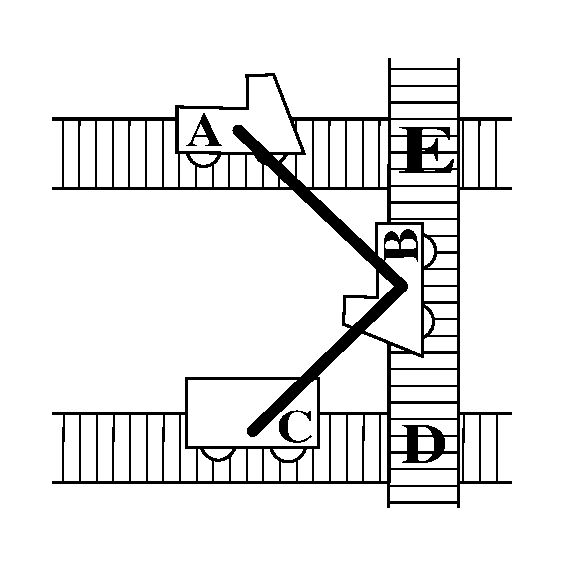
\includegraphics[width=3in]{trains.ps}\end{center}
\end{multicols}
\end{problem}

\begin{solution}
\subsection*{Solution}
I think the easiest way to think about this problem is as two ladder
problems, connected together.  We make some definitions:
\begin{eqnarray*}
a(t) &=& \mbox{the distance between Arthur and switch~E,} \\
b(t) &=& \mbox{the distance between Bertram and switch~E,} \\
c(t) &=& \mbox{the distance between Clarabel and switch~D,} \\
\end{eqnarray*}
Then the existence and tautness of 50 foot iron chain implies $a(t)^2
+ b(t)^2 = 50^2$, and differentiating with respect to time gives
$$
2 a(t) a'(t) + 2 b(t) b'(t) = 0.
$$
At the given time $t$, we are told $a(t) = 30$ and $a'(t) = 10$ and
$b(t) = 40$, so we solve and find
$$
b'(t) = \frac{- 2 \cdot 30 \cdot 10}{2 \cdot 40} = -60/8.
$$
Now the distance between Bertram and switch~D equals $70 - b(t)$,
so the 50 foot steel cable beween Bertram and Clarabel implies
$$
(70 - b(t))^2 + c(t)^2 = 50^2,
$$
and differentiating with respec to $t$ gives
$$
2 \, (70 - b(t)) \, (-b'(t)) + 2 \, c(t) \, c'(t) = 0.
$$
At the given time $t$, we are told $70 - b(t) = 30$ and $c(t) = 40$, and from our earlier calculation, $b'(t) = - 60/8$, so solving for $c'(t)$ gives
$$
c'(t) = \frac{-2 \cdot 30 \cdot 60 / 8}{2 \cdot 40} = \frac{-45}{8}.
$$
so Clarabel is moving toward switch~D at a rate of $45/8 = 5.625$
feet per minute.
\end{solution}




\end{document}
